% change according to folder and file names
\ifpdf
    \graphicspath{{5/figures/PNG/}{5/figures/PDF/}{4/figures/}}
\else
    \graphicspath{{5/figures/EPS/}{5/figures/}}
\fi

%: ----------------------- contents from here ------------------------
\chapter{Βελτιστοποίηση Υδροδυναμικών Στροβιλομηχανών}  % top level followed by section, subsection
Σκοπός αυτού του κεφαλαίου είναι να παρουσιάσει το κέρδος, σε μείωση υπολογιστικού κόστους, που επιτεύχθηκε από τη χρήση των προτεινόμενων σε αυτήν τη διατριβή μεθόδων σε προβλήματα βιομηχανικής κλίμακας και, ειδικότερα, στο σχεδιασμό υδροδυναμικών στροβιλομηχανών. Αναλυτικά θα παρουσιασθούν α) η χρήση \english{KBD} κατά το σχεδιασμό-βελτιστοποίηση ενός υδροστροβίλου τύπου \english{Francis} και β) η χρήση  εξελικτικών τελεστών υποβοηθούμενων από ΑσΚΣ, δηλαδή της μεθόδου που συμβολίζεται με ΜΑΕΑ\english{(PCA)} κατά το σχεδιασμό-βελτιστοποίηση ενός υδροστροβίλου τύπου \english{Hydromatrix\circledR}. 

Η διαδικασία παραμετροποίησης και αξιολόγησης των υποψηφίων λύσεων (μέσω της αριθμητικής επίλυσης των εξισώσεων \english{Euler}) είναι όμοια και για τους δύο τύπους στροβιλομηχανών και παρουσιάζεται με λεπτομέρεια στο πλήρες κείμενο της διατριβής.   

Όπως θα φανεί στη συνέχεια, είναι επιθυμητό η βελτιστοποίηση  να επιδιώξει την ελαχιστοποίηση αρκετών διαφορετικών συναρτήσεων που εκφράζουν την ποιότητα των σχεδιαζόμενων στροβιλομηχανών ή των συνιστωσών τους και, μάλιστα, σε περισσότερα του ενός σημεία λειτουργίας. Παρότι υπάρχει η δυνατότητα το χρησιμοποιούμενο λογισμικό βελτιστοποίησης (ΕΑ ή ΜΑΕΑ) να αναζητήσει μέτωπα \english{Pareto} στον πολυδιάστατο χώρο, εν τούτοις, για πρακτικούς λόγους θα χρησιμοποιηθούν ως συναρτήσεις κόστους κατάλληλοι συγκερασμοί των προαναφερθεισών ποσοτήτων στα διάφορα σημεία λειτουργίας. Έτσι, οι ποσότητες που μετρούν ποιότητα, ως προς διάφορα χαρακτηριστικά, θα αναφέρονται ως «μετρικές ποιότητας» (\english{quality metrics}) και δεσμεύεται η χρήση του όρου «συνάρτηση κόστους» για τις συναρτήσεις που ελαχιστοποιούνται από τον ΕΑ ή τον ΜΑΕΑ ή κάθε παραλλαγή τους.   
Οι τέσσερις μετρικές ποιότητας που χρησιμοποιούνται για να ποσοτικοποιήσουν την ποιότητα κάθε υποψήφιας λύσης είναι: 
\begin{itemize}
\item{\textbf{$\sigma$:}} Μετρική σπηλαίωσης η οποία εκφράζει την «απόσταση» από την κατάσταση εμφάνισης του φαινομένου της σπηλαίωσης. 
\item{\textbf{M$_1$:}} Μετρική καλής συνεργασίας με τον αγωγό απαγωγής, η οποία εκφράζει την απόκλιση της κατανομής της περιφερειακής $C_u$ και μεσημβρινής $C_m$ συνιστώσας της ταχύτητας στην είσοδο του αγωγού απαγωγής από κατανομές-στόχους που θέτει ο σχεδιαστής. Επιδιώκεται, προφανώς, η ελαχιστοποίηση των παραπάνω αποκλίσεων.
\item{\textbf{M$_2$:}} Μετρική ομοιόμορφης φόρτισης του πτερυγίου, μέσω της οποίας επιδιώκεται η, κατά το δυνατό, ομοιομορφία της φόρτισης του πτερυγίου κατά την κατεύθυνση της χορδής.
\item{\textbf{M$_3$:}} Μετρική επιφάνειας άντλησης. Στην περίπτωση μη-ρυθμιζόμενων υδροδυναμικών μηχανών, όπως ο \english{Hydromatrix\circledR}, δημιουργούνται περιοχές του πτερυγίου της κινητής πτερύγωσης όπου η πλευρά υπερπίεσης έχει χαμηλότερη πίεση  από την πλευρά υποπίεσης. Το φαινόμενο εμφανίζεται συνήθως κατά τη λειτουργία σε μερικό φορτίο και είναι επιθυμητό  η έκταση του να ελαχιστοποιηθεί.   
\end{itemize}

\section{Βελτιστοποίηση Υδροστροβίλου $Francis$}
Η ενότητα αυτή αναφέρεται στο σχεδιασμό-βελτιστοποίηση του δρομέα ενός υδροστροβίλου $Francis$, κάνοντας χρήση της τεχνικής \english{KBD}. Ο σχεδιασμός συμπεριλαμβάνει, για λόγους στιβαρότητας κατά τη λειτουργία, τρία σημεία λειτουργίας: τα σημεία  μερικού (ΜΦ) και πλήρους φορτίου (ΠΦ) και το σημείο μέγιστης απόδοσης (ΜΑ). Στο πρόβλημα εμπλέκονται δύο συναρτήσεις-στόχοι ανά σημείο λειτουργίας, οριζόμενες μέσω των μετρικών $M_1$ και $M_2$, ως εξής 

\begin{eqnarray}
   f_1^i=M_1^i ~~~\&~~~ f_2^i=M_2^i 
   \label{ObjFrancis} 
\end{eqnarray}
όπου ο άνω δείκτης $i=1,2,3$ χαρακτηρίζει το σημείο λειτουργίας.

Οι προαναφερθέντες $2\times3=6$ συναρτήσεις-στόχοι ομαδοποιούνται σε $2$ συναρτήσεις κόστους με τη σχέση    

\begin{eqnarray}
   f_1=\sum^3_{i=1}w_if_1^i ~~~\&~~~ f_2=\sum^3_{i=1}w_if_2^i 
   \label{ObjFrancis2} 
\end{eqnarray}
όπου $w_i$ καθοριζόμενος συντελεστής βάρους ανά σημείο λειτουργίας (πίνακας \ref{op-weights}).

\begin{table}[h!]
\begin{center}
\begin{tabular}{ |c|l| }
\hline
Σημείο Λειτουργίας & Βάρος $(w_i)$\\
\hline
Μέγιστης Απόδοσης (ΜΑ), $i=1$ & 1.0\\
\hline
Μερικού Φορτίου  (ΜΦ), $i=2$ & 0.3\\
\hline
Πλήρους Φορτίου (ΠΦ), $i=3$ & 0.3\\
\hline
\end{tabular}
\caption{Βελτιστοποίηση υδροστροβίλου $Francis$: Συντελεστές Βαρύτητας ανά σημείο λειτουργίας.}
\label{op-weights}
\end{center}
\end{table}

 Ο υδροστρόβιλος $Francis$ έχει ρυθμιζόμενα οδηγά περύγια άρα η μετρική της επιφάνειας άντλησης ($Μ_3$) δεν χρειάζεται να χρησιμοποιηθεί. Έτσι όπως διατυπώθηκε το πρόβλημα, η μετρική που αφορά στη σπηλαίωση (σ) αλλά και το επιθυμητό υδραυλικό ύψος (Η) χρησιμοποιήθηκαν ως περιορισμοί (πίνακας \ref{Cons}).


\begin{table}[h!]
\begin{center}
\begin{tabular}{ |c|c|c| }
\hline
Σημείο Λειτουργίας  & $\sigma_i^{Hist}<\sigma$ & Υδραυλικό ύψος\\
\hline
ΜΑ & $\sigma_i^{Hist}<0.2$ & $|\Delta H|<1.5\%$\\
\hline
ΜΦ       & $\sigma_i^{Hist}<0.2$ & $|\Delta H|<5\%$\\
\hline
ΠΦ       & $\sigma_i^{Hist}<0.2$ & $|\Delta H|<5\%$\\
\hline
\end{tabular}
\caption{Βελτιστοποίηση υδροστροβίλου $Francis$: Τεθέντες περιορισμοί, σχετικοί με τη σπηλαίωση (στη μορφή της μετρικής σ, ορισμός του $\sigma_i^{Hist}$ υπάρχει στο πλήρες κείμενο της διατριβής) και το υδραυλικό ύψος Η, στα τρία σημεία λειτουργίας. Η ποσότητα $|\Delta H|$ εκφράζει την απόλυτη τιμή της διαφοράς του ύψους Η από την επιθυμητή τιμή αυτού στο κάθε σημείο λειτουργίας. Με τις χρησιμοποιούμενες οριακές συνθήκες, η ανάλυση της ροής στο δρομέα με λογισμικό ΥΡΔ έχει ως εξαγόμενο το υδραυλικό ύψος Η το οποίο, σε κάθε σημείο λειτουργίας, οφείλει να έχει δεδομένη τιμή, με επιθυμητή ανοχή $|\Delta H|$.}
\label{Cons}
\end{center}
\end{table}


Η γεωμετρία του προς βελτιστοποίηση δρομέα παραμετροποιείται με $336$ μεταβλητές σχεδιασμού, όπως αυτές παρουσιάζονται στο αντίστοιχο κεφάλαιο του πλήρους κειμένου της διατριβής. 


\subsection{Αρχειοθετημένοι Σχεδιασμοί Βάσης}
Για την υποστήριξη της διαδικασίας σχεδιασμού-βελτιστοποίησης με τη μέθοδο $KBD$, εντοπίστηκαν τρεις ($m\!=\!3$) αρχειοθετημένοι σχεδιασμοί, οι οποίοι σχεδιάστηκαν στο παρελθόν για «κοντινά», σε σχέση με το επιθυμητό, σημεία λειτουργίας. Αυτοί οι σχεδιασμοί χρησιμοποιούνται  ως σχεδιασμοί βάσης κατά την εφαρμογή της μεθόδου \english{KBD}. Οι επιδόσεις των σχεδιασμών βάσης στα επιθυμητά σημεία λειτουργίας παρουσιάζονται στον πίνακα \ref{reuse}.

\begin{table}[h!]
\begin{center}
\begin{tabular}{ |c|c|c|c|c|c| }
\hline
Σχεδιασμός & ΣΛ & $M_1$ & $M_2$  & $\sigma_i^{Hist}$ & $|\Delta H|$\\
Βάσης & & & & &\\
\hline
Β1 & ΜΑ & $0.472$ & $0.538$ & $0.21 >0.2$ * & $ 5\% >1.5\%$ * \\
Β1 & ΜΦ & $0.552$ & $0.824$ & $0.23 > 0.2$ * & $ 3.6\% <5\%$ \\
Β1 & ΠΦ & $0.408$ & $0.594$ & $0.2 = 0.2$  & $ 5.7\% >5\%$ * \\
\hline
\hline
Β2 & ΜΑ & $0.563$ & $0.922$ & $0.22 > 0.2$ * & $ 3.8\% >1.5\%$ * \\
Β2 & ΜΦ & $0.534$ & $0.888$ & $0.24 > 0.2$ * & $ 2.6\% <5\%$  \\
Β2 & ΠΦ & $0.522$ & $1.178$ & $0.22 > 0.2$ * & $ 4.8\% <5\%$  \\
\hline
\hline
Β3 & ΜΑ & $0.402$ & $0.663$ & $0.19 < 0.2$  & $ 6.8\% >1.5\%$ * \\
Β3 & ΜΦ & $0.515$ & $0.808$ & $0.21 > 0.2$ * & $ 6.9\% >5\%$ * \\
Β3 & ΠΦ & $0.257$ & $0.896$ & $0.18 < 0.2$  & $ 7.1\% >5\%$ * \\
\hline
\end{tabular}
\caption{Βελτιστοποίηση Υδροστροβίλου $Francis$: Οι μετρικές ποιότητας ($M_1$ και $M_2$) που σχηματίζουν τους στόχους και οι περιορισμοί (σ και $|\Delta H|$) για τους σχεδιασμούς βάσης ($B1, B2$ και $B3$) για τα επιθυμητά σημεία λειτουργίας. Ο αστερίσκος (*) στους περιορισμούς υποδηλώνει ότι ο υπόψη σχεδιασμός βάσης παραβιάζει τον αντίστοιχο περιορισμό.}
\label{reuse}
\end{center}
\end{table}

\begin{figure}[h!]
\begin{minipage}[b]{0.5\linewidth}
 \centering
 \resizebox*{6.5cm}{!}{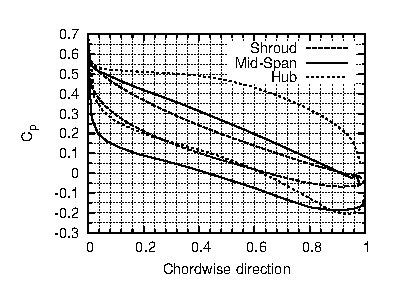
\includegraphics{Load_B1.eps}}
\end{minipage}
\begin{minipage}[b]{0.5\linewidth}
 \centering
 \resizebox*{6.5cm}{!}{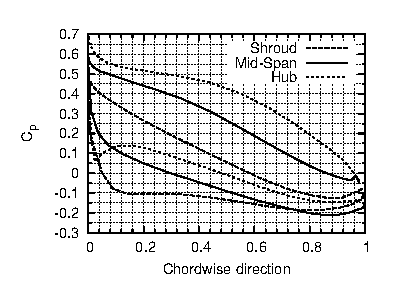
\includegraphics{Load_B2.eps}}
\end{minipage}
\begin{minipage}[b]{1\linewidth}
 \centering
 \resizebox*{6.5cm}{!}{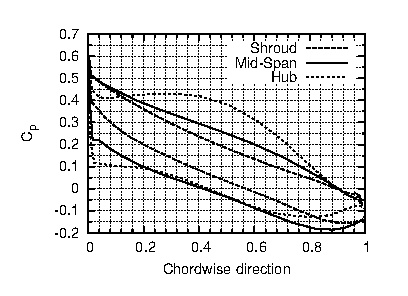
\includegraphics{Load_B3.eps}}
\end{minipage}
\caption{Βελτιστοποίηση υδροστροβίλου $Francis$: Κατανομές του συντελεστή πίεσης $C_p$ κατά μήκος της χορδής για τρεις χαρακτηριστικές καθ' ύψος  θέσεις στο πλήμνη , \english{(hub)}, μέσο ύψος \english{(mid-span)} και στεφάνη \english{(shroud)}  για τους σχεδιασμούς βάσης, Β1 (πάνω-αριστερά), Β2 (πάνω-δεξιά) και Β3 (κάτω).}
\label{Francis-LOAD}
\end{figure}


Η ποιότητα των σχεδιασμών βάσης, όταν αυτοί χρησιμοποιηθούν στα επιθυμητά σημεία, είναι αρκετά κακή όπως φαίνεται στον πίνακα \ref{reuse}. Αυτό γίνεται ακόμη πιο εμφανές από τα σχήματα \ref{Francis-LOAD}, όπου φαίνεται η ανομοιομορφία φόρτισης των πτερυγίων του δρομέα, και \ref{Francis-OUT}, όπου φαίνεται η μεγάλη απόκλιση από τις κατανομές-στόχους της περιφερειακής και μεσημβρινής ταχύτητας στην έξοδο, άρα και η κακή συνεργασία που θα είχαν με τον αγωγό απαγωγής.         


\begin{figure}[h!]
\begin{minipage}[b]{0.5\linewidth}
 \centering
 \resizebox*{6cm}{!}{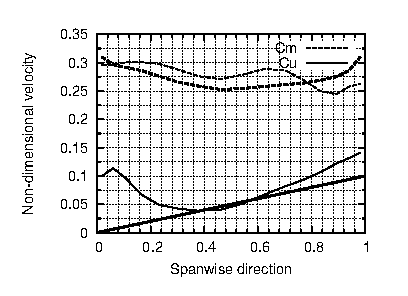
\includegraphics{OUTLET_B1.eps}}
\end{minipage}
\begin{minipage}[b]{0.5\linewidth}
 \centering
 \resizebox*{6cm}{!}{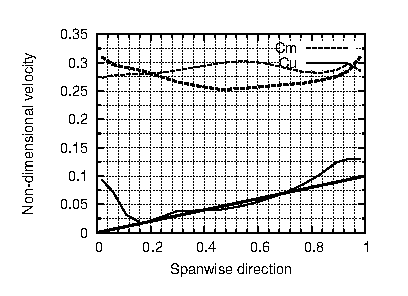
\includegraphics{OUTLET_B2.eps}}
\end{minipage}
\begin{minipage}[b]{1\linewidth}
 \centering
 \resizebox*{6cm}{!}{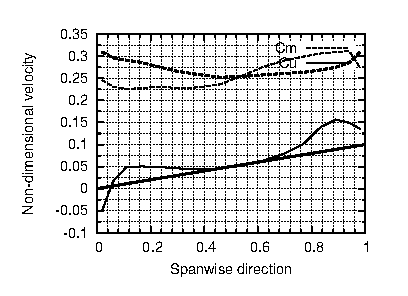
\includegraphics{OUTLET_B3.eps}}
\end{minipage}
\caption{Βελτιστοποίηση υδροστροβίλου $Francis$: Κατανομές περιφερειακής ($C_u$) και μεσημβρινής ($C_m$)  συνιστώσας της ταχύτητας εξόδου για τους σχεδιασμούς βάσης, Β1 (πάνω-αριστερά), Β2 (πάνω-δεξιά) και Β3 (κάτω) σε αντιπαραβολή με τις αντίστοιχες κατανομές-στόχους που καθορίστηκαν από το σχεδιαστή.}
\label{Francis-OUT}
\end{figure}

Κατά την εφαρμογή της μεθόδου $KBD$, οι μεταβλητές σχεδιασμού ομαδοποι-ούνται σε $6$ ομάδες και, μαζί με τη μεταβλητή  προεκβολής
$\Psi$, δημιουργούν τις $19$ ($=3\times6+1$) μεταβλητές βελτιστοποίησης. Η λεπτομερής ομαδοποίηση περιγράφεται στο πλήρες κείμενο της διατριβής. Είναι, εκ των πραγμάτων, συγκριτικά πλεονεκτικότερη η χρήση ΕΑ (ή ΜΑΕΑ) για την αναζήτηση του βέλτιστου συνόλου των $19$, αντί των $336$ (της κανονικής παραμετροποίησης), μεταβλητών.   

\subsection{Αποτελέσματα - Συγκρίσεις}
Ο σχεδιασμός πραγματοποιήθηκε κάνοντας χρήση ενός ΕΑ και ενός ΜΑΕΑ(\english{KBD}). Ο ρυθμός σύγκλισης των συναρτήσεων κόστους, σε κάθε περίπτωση παρουσιάζεται στο σχήμα \ref{Francis-Res}, όπου σχεδιάζεται ο δείκτης υπερόγκου (\english{hypervolume indicator}, \cite{Zitz2007}). Στο συμβατικό ΕΑ ήταν ιδιαίτερα αναποτελεσματική η χρήση μεταπροτύπων με αποδοτικό τρόπο λόγω του μεγάλου αριθμού μεταβλητών σχεδιασμού ($336$), όπως άλλωστε παρατηρήθηκε και κατά την εφαρμογή της ενότητας \ref{Drela1}. Αντίθετα, κάνοντας χρήση της μεθόδου \english{KBD} γίνεται ξανά δυνατή η χρήση μεταπροτύπων μέσω της τεχνικής ΠΠΑ, η οποία ξεκινά όταν στη βάση δεδομένων του ΜΑΕΑ αποθηκευθούν $150$ (μη-τιμωρημένα με «ποινή θανάτου») άτομα. Η ρύθμιση των παραμέτρων των δύο ΕΑ παρουσιάζεται στο πλήρες κείμενο της διατριβής. Και στις δύο διαδικασίες βελτιστοποίησης, οι 3 σχεδιασμοί βάσης επιβάλλονται ως μέλη του πληθυσμό της πρώτης γενιάς του ΕΑ.      
          
\begin{figure}[h!]
\begin{minipage}[b]{0.5\linewidth}
 \centering
 \resizebox*{7.0cm}{!}{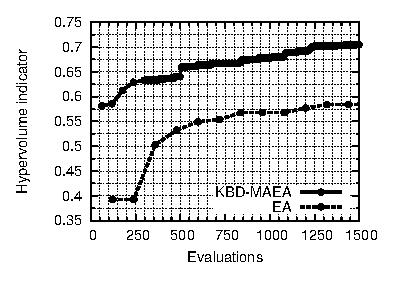
\includegraphics{HypComp.eps}}
\end{minipage}
\begin{minipage}[b]{0.5\linewidth}
 \centering
 \resizebox*{7.0cm}{!}{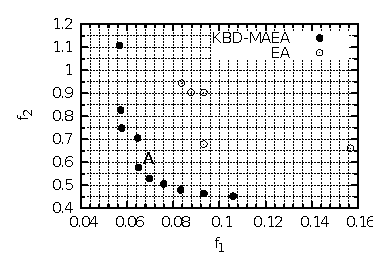
\includegraphics{Comp.eps}}
\end{minipage}
\caption{Βελτιστοποίηση υδροστροβίλου $Francis$:  Σύγκριση πορείας του δείκτη υπερόγκου για τη δικριτηριακή βελτιστοποίηση με ΕΑ και ΜΑΕΑ(\english{KBD}) (αριστερά). Μέτωπα μη-κυριαρχούμενων λύσεων (για Μ=$2$) για τους ΕΑ και ΜΑΕΑ(\english{KBD}) που υπολογίστηκαν έχοντας ως κριτήριο τερματισμού τις $1500$ αξιολογήσεις με το λογισμικό ΥΡΔ (δεξιά).}
\label{Francis-Res}
\end{figure}

Είναι εμφανές (σχήμα \ref{Francis-Res}, αριστερά) ότι η προτεινόμενη μέθοδος, ΜΑΕΑ(\english{KBD}): α) εκκινεί από υψηλότερη τιμή του δείκτη υπερόγκου κάτι που υποδηλώνει ότι ο τρόπος  καθορισμού σημαντικότητας στις περιοχές του χώρου σχεδιασμού είναι πολύ κοντά στη φυσική του προβλήματος και β) συνεχίζει με συνεχώς καλύτερες τιμές για όλη τη διάρκεια της βελτιστοποίησης. Η ανωτερότητα της μεθόδου \english{KBD} γίνεται ακόμη περισσότερο εμφανής παρατηρώντας τα τελικά μέτωπα των μη-κυριαρχούμενων λύσεων τα οποία αντιστοιχούν στο ίδιο υπολογιστικό κόστος ($1500$ αξιολογήσεις) (σχήμα \ref{Francis-Res}, δεξιά). Τέλος, από το μέτωπο των μη-κυριαρχούμενων λύσεων που προέκυψε από το       ΜΑΕΑ(\english{KBD}), επιλέγεται το άτομο Α το οποίο και αναλύεται περαιτέρω στη συνέχεια (σχήμα \ref{design-bases-a}).


\begin{figure}[h!]
\begin{minipage}[b]{1\linewidth}
 \centering
 \resizebox*{10.0cm}{!}{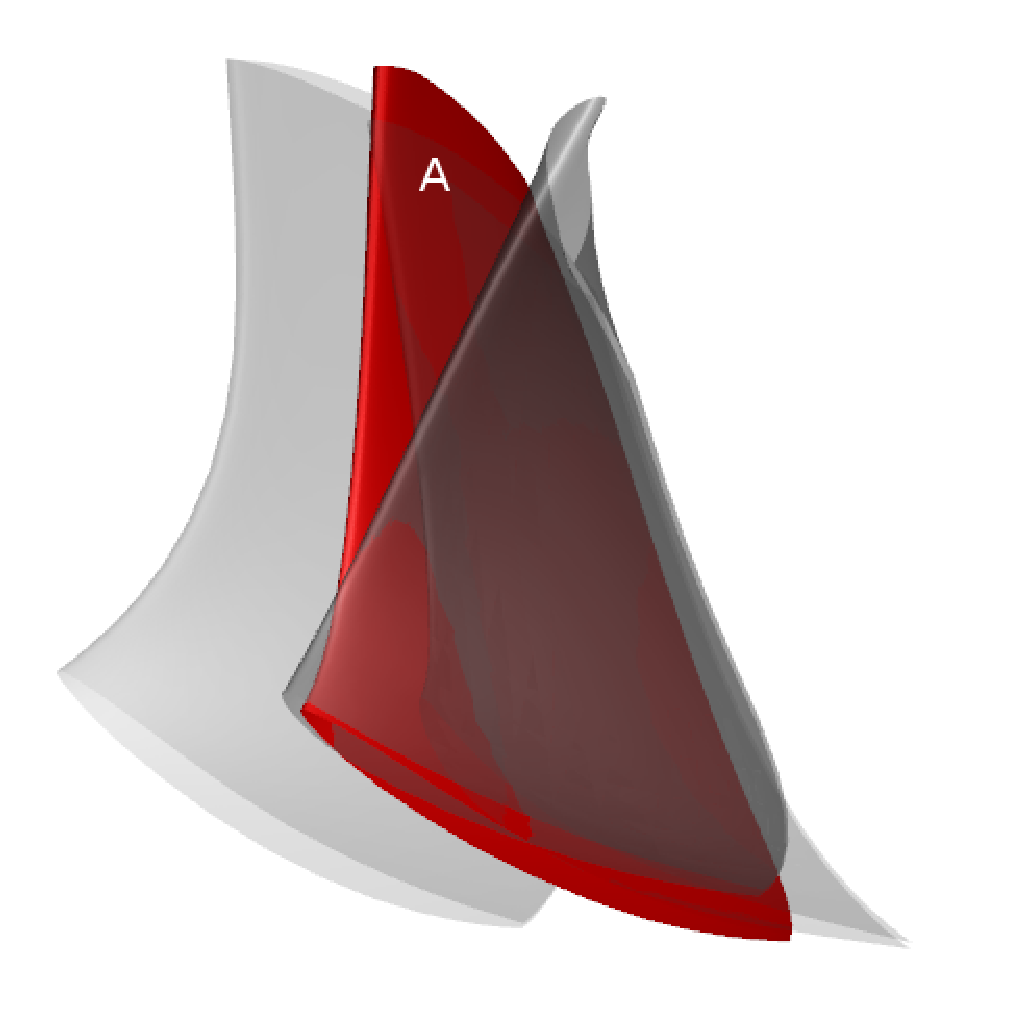
\includegraphics{final.eps}}
\end{minipage}
\caption{Βελτιστοποίηση υδροστροβίλου $Francis$: Το πτερύγιο του δρομέα του επιλεγμένου σχεδιασμού Α και οι τρεις σχεδιασμοί βάσης που χρησιμοποιήθηκαν.}
\label{design-bases-a}
\end{figure}

\begin{table}[h!]
\begin{center}
\begin{tabular}{ |c|c|c|c|c|c| }
\hline
Σχεδιασμός & ΣΛ & $M_1$ & $M_2$  &  $\sigma_i^{Hist}$ & $|\Delta H|$\\
\hline
A & ΜΑ & $0.001$ & $0.302$ & $0.18 < 0.2$ & $ 1.1\% <1.5\%$ \\
A & ΜΦ & $0.086$ & $0.409$ & $0.19 < 0.2$ & $ 1.5\% <5\%$ \\
A & ΠΦ & $0.092$ & $0.504$ & $0.18 < 0.2$ & $ 4.1\% <5\%$  \\
\hline
\end{tabular}
\caption{Βελτιστοποίηση υδροστροβίλου $Francis$: Οι μετρικές ποιότητας ($M_1$ και $M_2$) που σχηματίζουν τους στόχους και οι περιορισμοί (σ και $|\Delta H|$) για το σχεδιασμό Α για τα τρία  υπόψη σημεία λειτουργίας (ΜΑ, ΜΦ και ΠΦ). Ο σχεδιασμός Α ικανοποιεί όλους τους περιορισμούς.}
\label{Asum}
\end{center}
\end{table}

Οι κατανομές του συντελεστή πίεσης $C_p$ σχεδιασμένες στις επιφάνειες του δρομέα του σχεδιασμού Α, στα τρία σημεία λειτουργίας, παρουσιάζονται στο σχήμα \ref{Francis-A}. Επιπλέον, για το σημείο ΜΑ, παρουσιάζονται και αναλυτικά οι κατανομές $C_p$ (σχήμα \ref{Francis-A-cp}, αριστερά) σχεδιασμένες στο πλήμνη , \english{(hub)}, στο μέσο ύψος \english{(mid-span)} και στην στεφάνη \english{(shroud)} της πτερύγωσης. Είναι εμφανής η ποιότητα του σχεδιασμού τόσο όσον αφορά στην ισοκατανεμημένη φόρτιση όσο και στην ασφάλεια από σπηλαίωση. Ακόμη, παρουσιάζονται κατανομές $C_u$ και $C_m$ στην έξοδο (σχήμα \ref{Francis-A-cp}, δεξιά) μαζί με τις κατανομές-στόχους.

\begin{figure}[h!]
\begin{minipage}[b]{0.5\linewidth}
 \centering
 \resizebox*{6cm}{!}{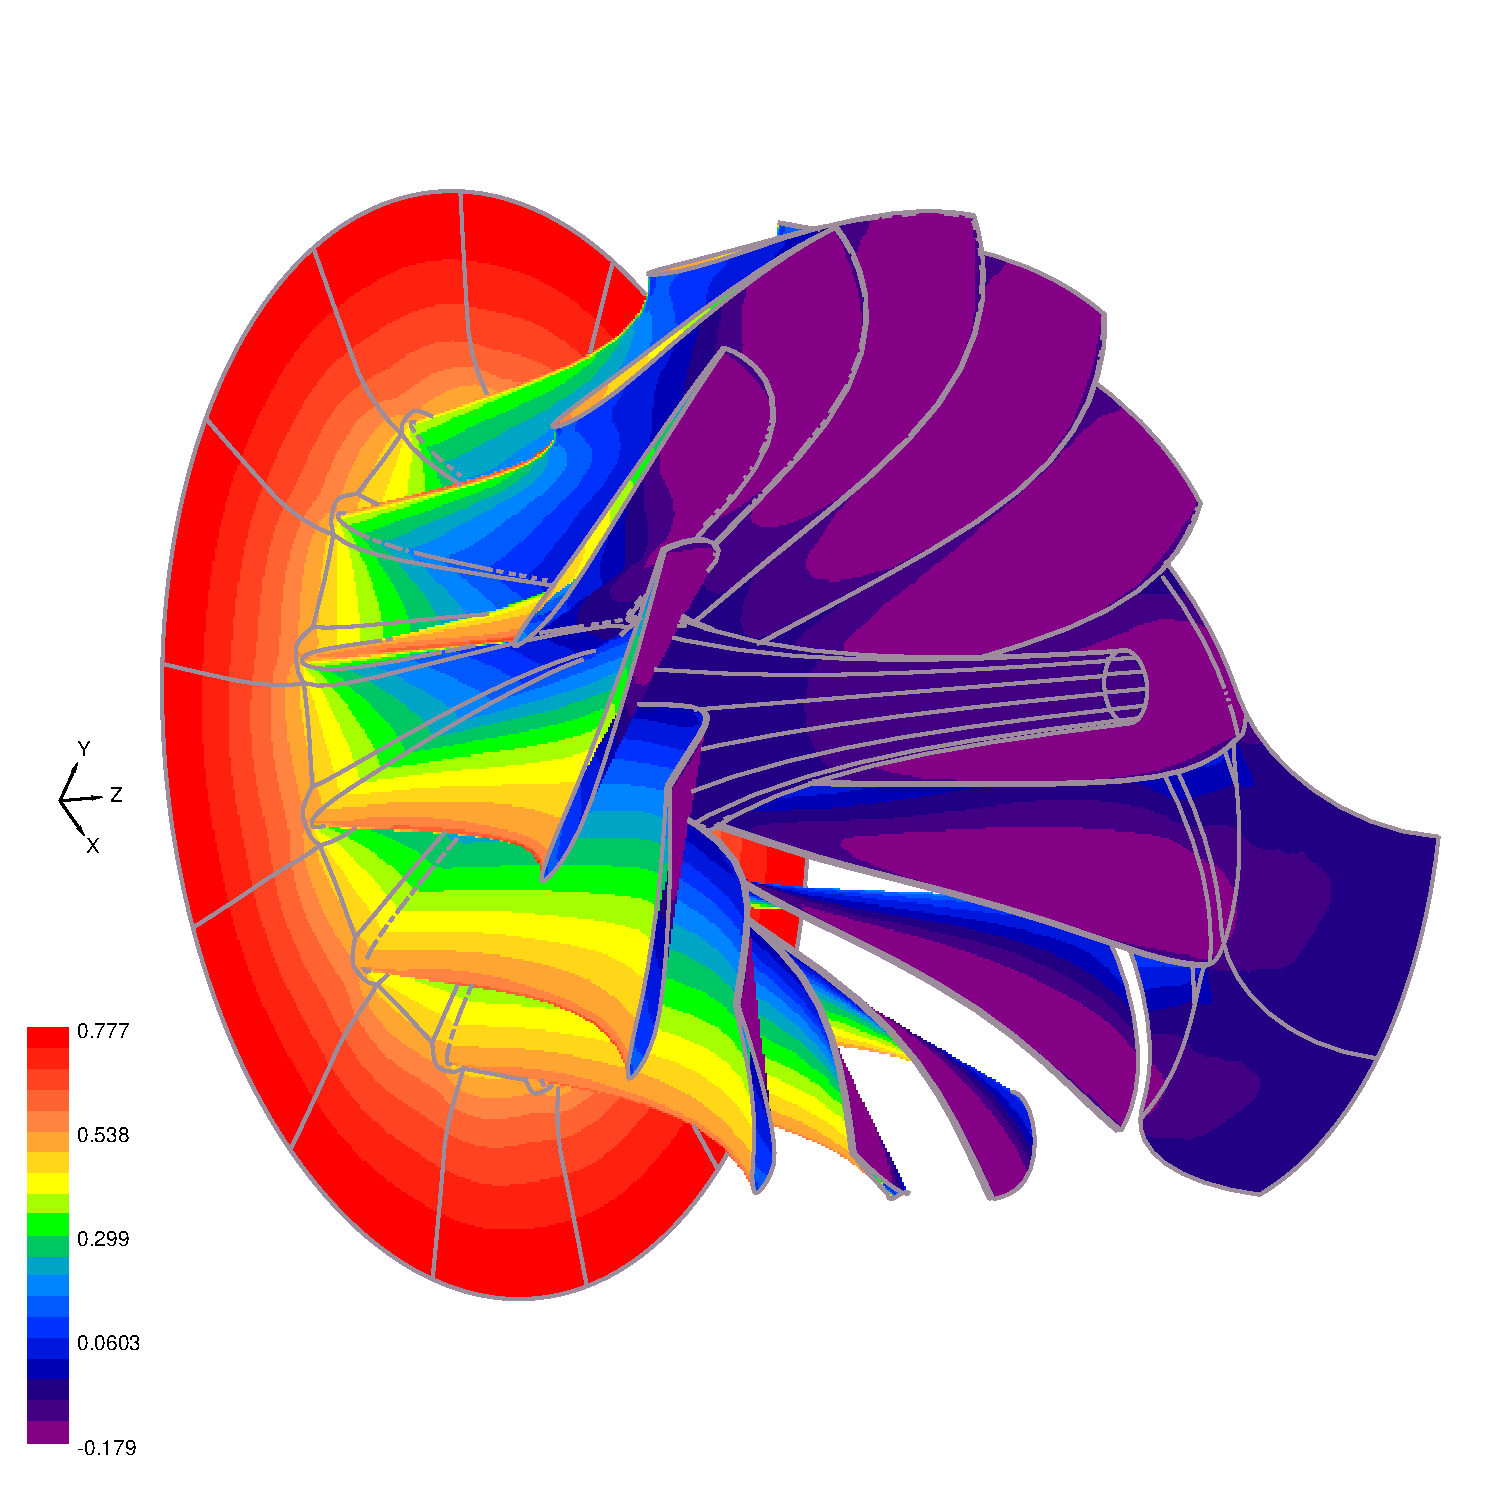
\includegraphics{ABE.eps}}
\end{minipage}
\begin{minipage}[b]{0.5\linewidth}
 \centering
 \resizebox*{6cm}{!}{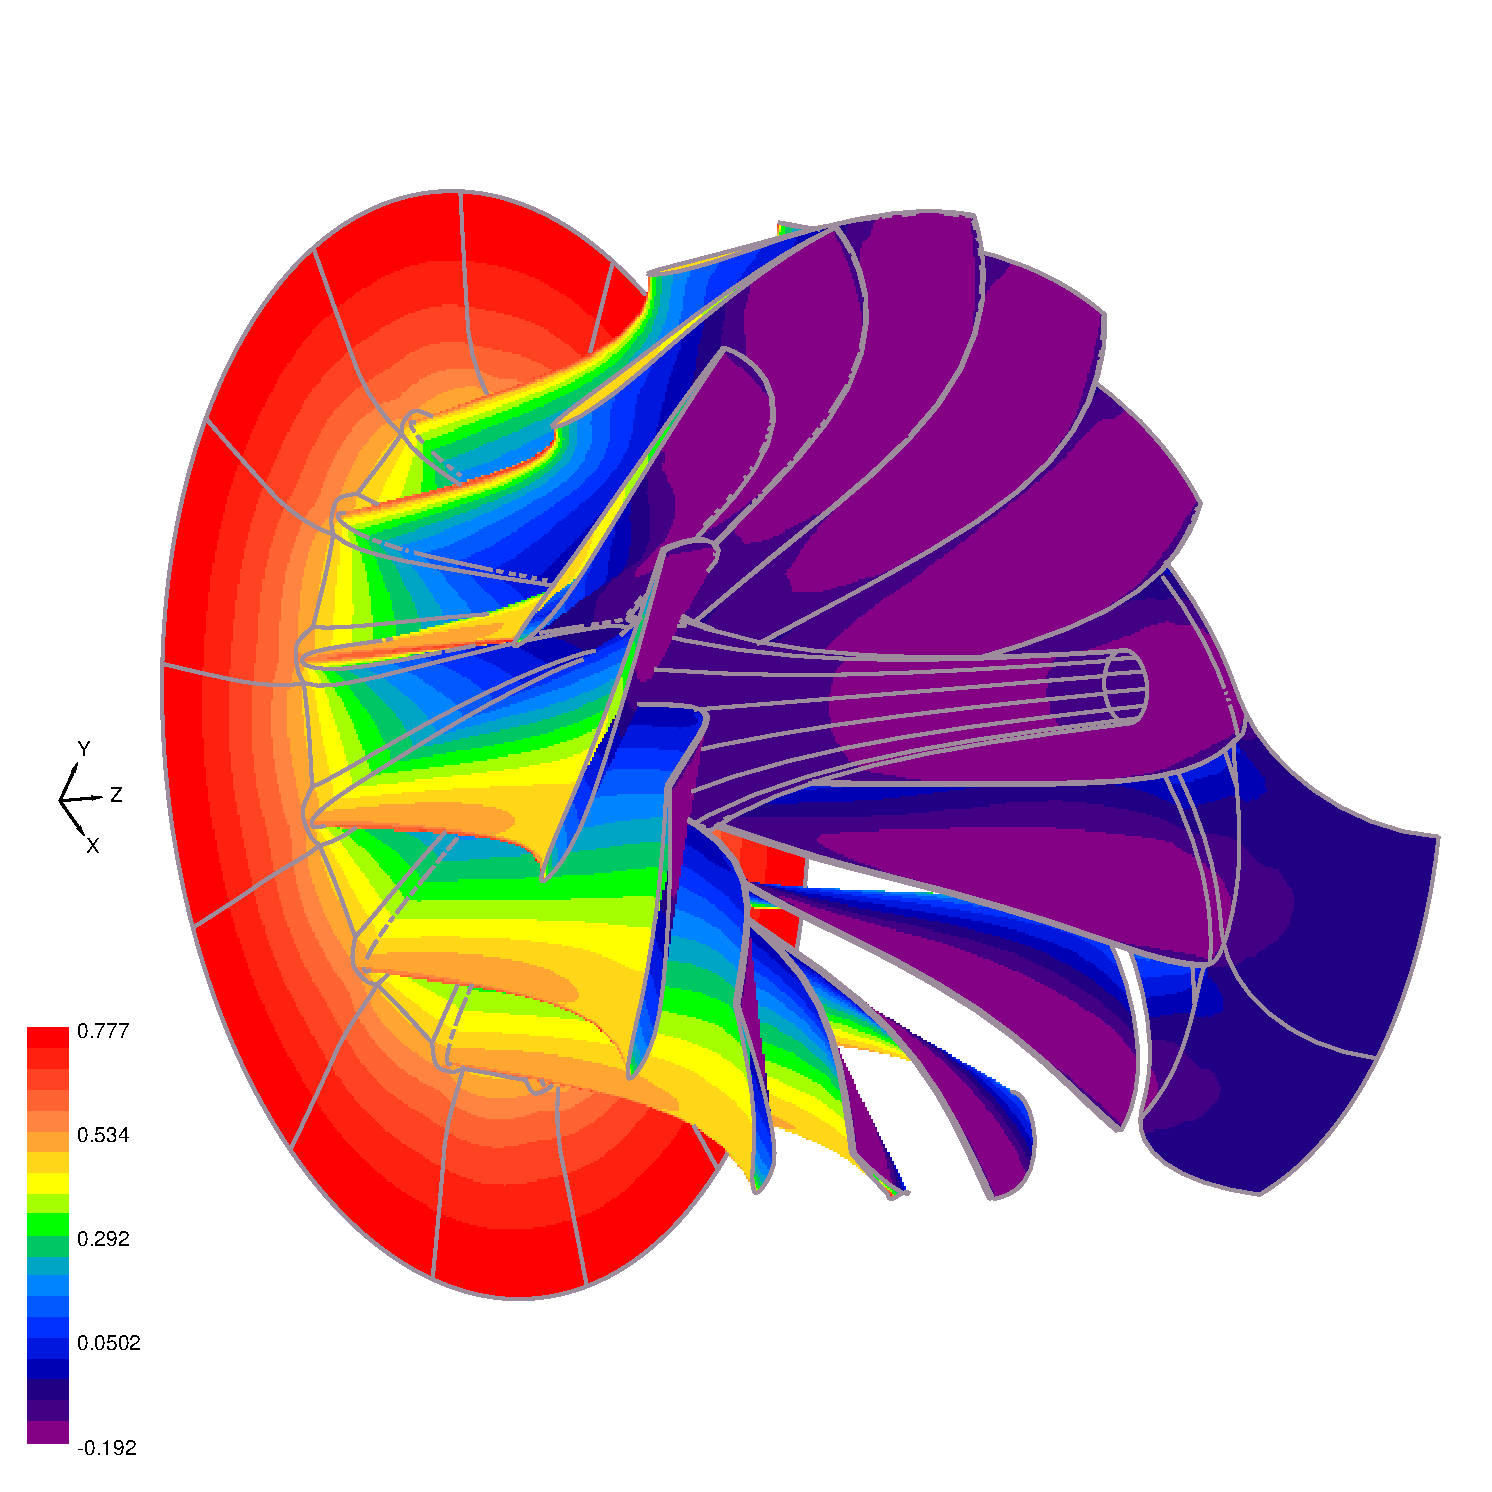
\includegraphics{APL.eps}}
\end{minipage}
\begin{minipage}[b]{1\linewidth}
 \centering
 \resizebox*{6cm}{!}{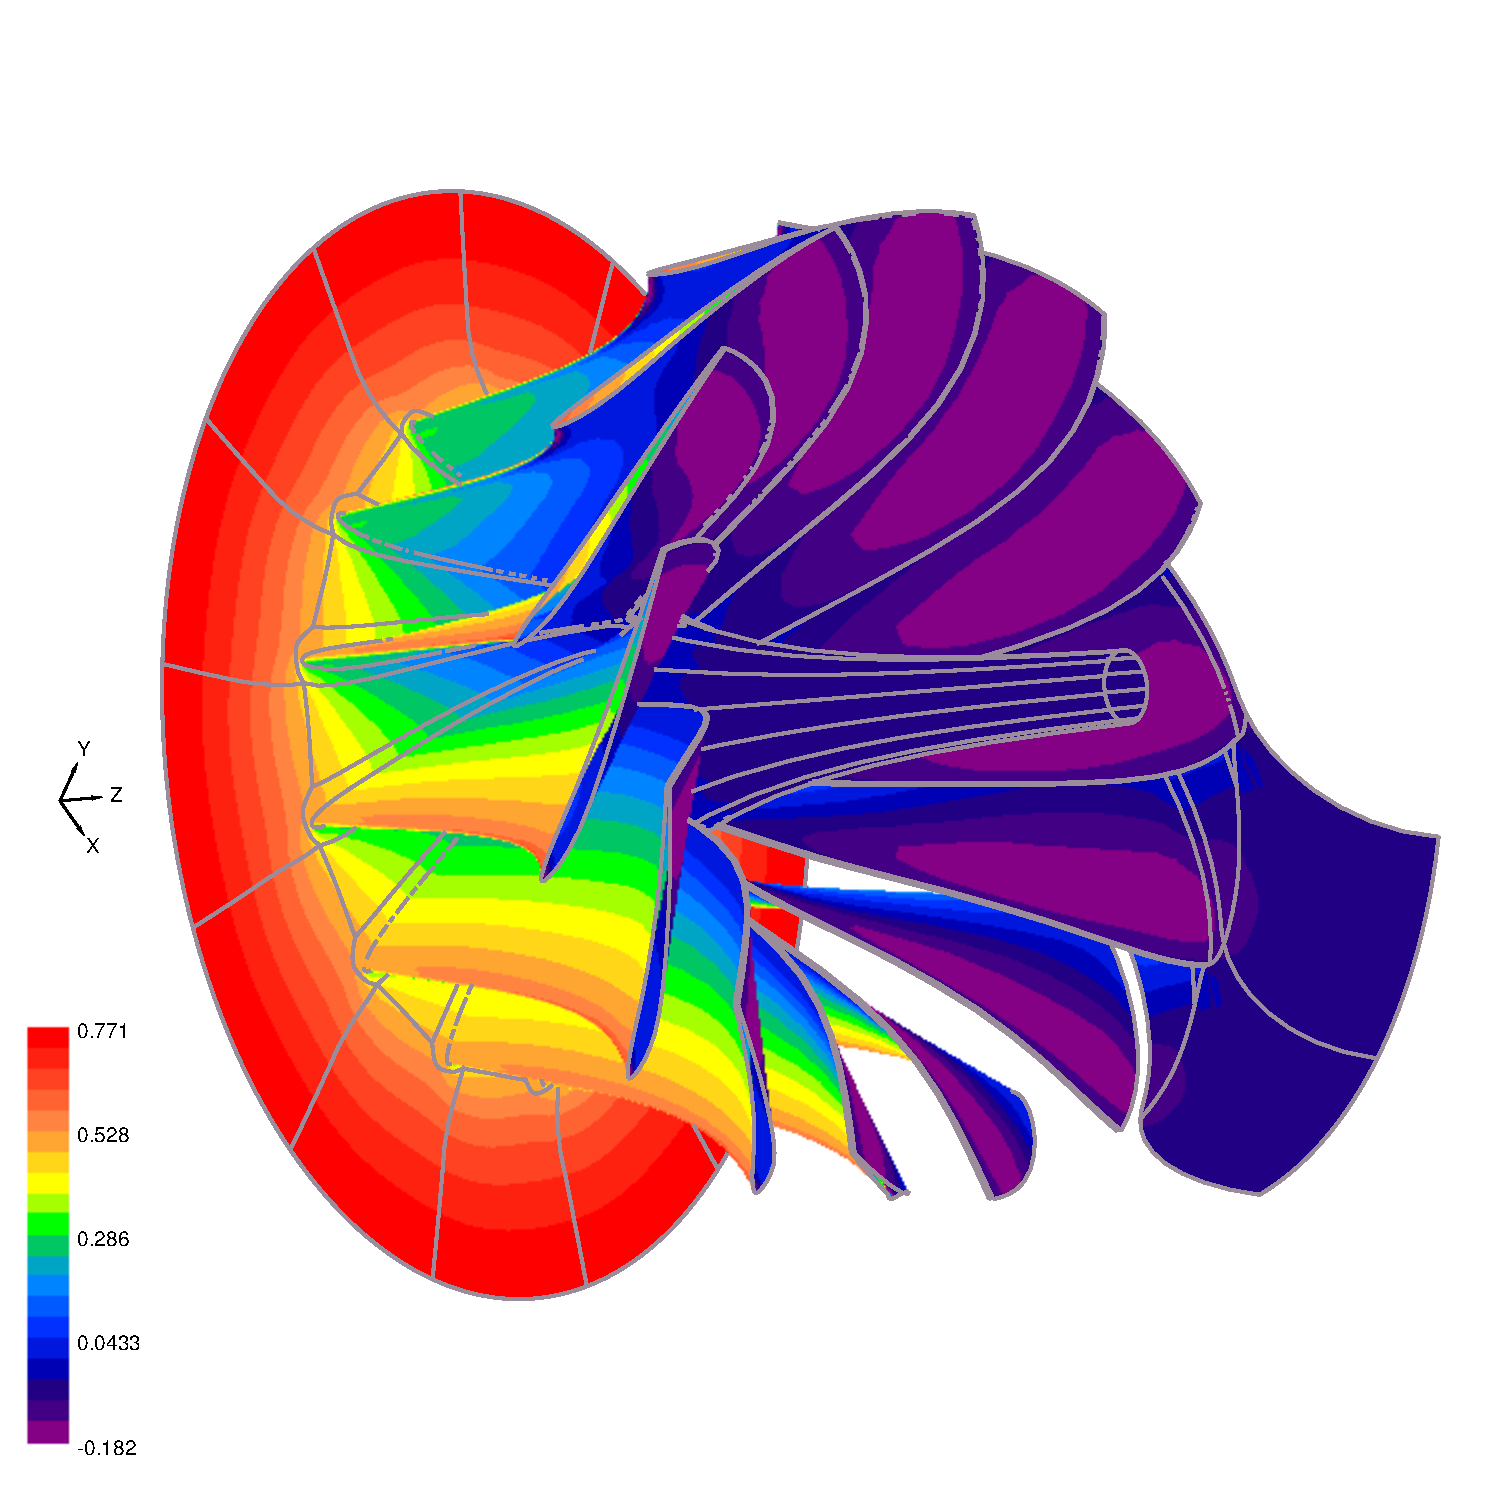
\includegraphics{AFL.eps}}
\end{minipage}
\caption{Βελτιστοποίηση υδροστροβίλου $Francis$: Κατανομές $C_p$ στο δρομέα του σχεδιασμού Α στα τρία σημεία λειτουργίας: ΜΑ (πάνω-αριστερά), ΜΦ (πάνω-δεξιά) και ΠΦ (κάτω).}
\label{Francis-A}
\end{figure}


\begin{figure}[h!]
\begin{minipage}[b]{0.5\linewidth}
 \centering
 \resizebox*{6.5cm}{!}{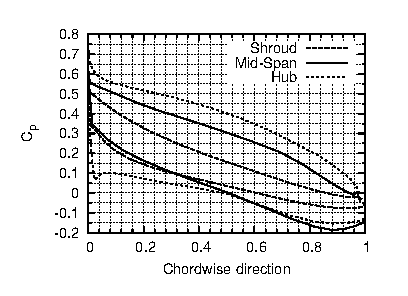
\includegraphics{Load_A.eps}}
\end{minipage}
\begin{minipage}[b]{0.5\linewidth}
 \centering
 \resizebox*{6cm}{!}{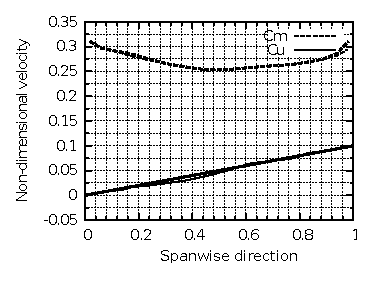
\includegraphics{OUTLET_A.eps}}
\end{minipage}
\caption{Βελτιστοποίηση υδροστροβίλου $Francis$:  Κατανομές $C_p$ για το δρομέα του σχεδιασμού Α στο σημείο ΜΑ (αριστερά). Κατανομές των συνιστωσών της ταχύτητας εξόδου $C_u$ και $C_m$ για το σχεδιασμό Α στο σημείο ΜΑ (δεξιά).}
\label{Francis-A-cp}
\end{figure}

\FloatBarrier

\section{Βελτιστοποίηση Υδροστροβίλου $Hydromatrix\circledR$}

Η ενότητα αυτή παρουσιάζει το σχεδιασμό-βελτιστοποίηση ενός υδροστροβίλου $Hydromatrix\circledR$ κάνοντας χρήση ΕΑ με τους υποβοηθούμενους από ΑσΚΣ εξελικτικούς τελεστές, δηλαδή της μεθόδου που αναφέρεται ως ΜΑΕΑ(\english{PCA}). Ο σχεδιασμός γίνεται σε τρία σημεία λειτουργίας: το σημείο μέγιστης απόδοσης (ΜΑ) και τα σημεία πλήρους (ΠΦ) και μερικού (ΜΦ) φορτίου. Ο συνδυασμός των μετρικών ποιότητας σε δύο  στόχους ανά σημείο λειτουργίας γίνεται με άθροισμα μέσω συντελεστών βαρύτητας (πίνακας \ref{op-weights-M1}), ως


\begin{eqnarray}
   f_1^i=\alpha ^i  M_1^i ~~~,~~~ f_2^i=\beta ^i Μ_2^i+\gamma ^i  \sigma_i^{Hist} +\delta ^i  Μ_3^i 
   \label{ObjFrancis} 
\end{eqnarray}
όπου ο άνω δείκτης $i=1,2,3$ αναφέρεται στο σημείο λειτουργίας.


\begin{table}[h!]
\begin{center}
\begin{tabular}{ |l|r|r|r|c| }
%\hline
%\multicolumn{4}{|c|}{Βάρη} & F \\
\hline
& ΜΑ, $i\!=\!1$ & ΜΦ, $i\!=\!2$ & ΠΦ, $i\!=\!3$ &  Στόχος\\
\hline
α ($M_1$) & 1.0            &0.0            &0.0 & $f_1$\\
\hline
β ($M_2$) &0.2    &0.0            &0.0  & $f_2$\\
\hline
γ ($\sigma_i^{Hist}$) &1.0            &1.0            &1.0 & $f_2$\\
\hline
δ ($M_3$) &0.0            &100.0  &100.0 & $f_2$\\
\hline
\end{tabular}
\caption{Βελτιστοποίηση υδροστροβίλου $Hydromatrix\circledR$: Συντελεστές βαρύτητας κατά την ομαδοποίηση των μετρικών σε δύο στόχους ανά σημείο λειτουργίας.}
\label{op-weights-M1}
\end{center}
\end{table}

 Ο συνδυασμός των συναρτήσεων-στόχων $f^i_1$ και $f^i_2$ για όλα τα σημεία λειτουργίας σε δύο, τελικά, συναρτήσεις-κόστους (M=$2$) γίνεται μέσω των συντελεστών βαρύτητας $w_i$ του πίνακα \ref{op-weights-M2} ως

\begin{eqnarray}
   f_1=\sum^3_{i=1}w_if_1^i ~~~,~~~ f_2=\sum^3_{i=1}w_if_2^i 
   \label{ObjFrancis2} 
\end{eqnarray}

\begin{table}[h!]
\begin{center}
\begin{tabular}{ |c|l| }
\hline
Σημείο λειτουργίας & $w_i$\\
\hline
Μέγιστης Απόδοσης (ΜΑ), $i\!=\!1$  & 1.0\\
\hline
Μερικού Φορτίου  (ΜΦ), $i\!=\!2$ & 0.1\\
\hline
Πλήρους Φορτίου (ΠΦ), $i\!=\!3$  & 0.1\\
\hline
\end{tabular}
\caption{Βελτιστοποίηση υδροστροβίλου $Hydromatrix\circledR$: Συντελεστές βαρύτητας $w_i$ ανά σημείο λειτουργίας.}
\label{op-weights-M2}
\end{center}
\end{table}

Στο παρόν πρόβλημα βελτιστοποίησης η μετρική που αφορά στη σπηλαίωση αναβαθμίζεται από περιορισμό σε μια από τις συνιστώσες της $f_2$. Επίσης, ο περιορισμός που αφορά στη λειτουργία στο επιθυμητό σημείο λειτουργίας δεν υφίσταται για το σημείο ΜΑ αφού, για κάθε υποψήφια λύση, πραγματοποιείται μια δεύτερη εσωτερική διαδικασία βελτιστοποίησης η οποία ρυθμίζει τη γωνία μετάλλου στην έξοδο της σταθερής πτερύγωσης ούτως ώστε ο σχεδιασμός να λειτουργεί στο επιθυμητό σημείο. Παρόλα αυτά, παραμένει απαραίτητη η χρήση του σχετικού περιορισμού που αφορά στη λειτουργία στα υπόλοιπα δύο σημεία λειτουργίας. Συγκεκριμένα, ο περιορισμός αυτός αφορά στην επιθυμητή παροχή όγκου, επιτρέποντας ποσοστιαία απόκλιση  της παροχής όγκου ρευστού $|\Delta Q| < 5\%$, κατ' αντιστοιχία με τους περιορισμούς $|\Delta Η|$ της προηγούμενης ενότητας.  Σημειώνεται ότι η ανάλυση της ροής στο δρομέα με λογισμικό ΥΡΔ έχει, σύμφωνα με τις επιβαλλόμενες οριακές συνθήκες, ως δεδομένο το ύψος Η και ως εξαγόμενο την παροχή $Q$.
              

\subsection{Αποτελέσματα - Συγκρίσεις}
Ό σχεδιασμός πραγματοποιήθηκε κάνοντας χρήση ενός MAΕΑ και ενός ΜΑΕΑ(\english{PCA}). Οι πορείες σύγκλισης των δύο παρουσιάζονται στο σχήμα \ref{Matrix-Res} χρησιμοποιώντας το δείκτη υπερόγκου, \cite{Zitz2007}, ως κριτήριο σύγκρισης.  Η ακριβής ρύθμιση των παραμέτρων των δύο δικριτηριακών MAΕΑ που δοκιμάστηκαν παρουσιάζεται στο πλήρες κείμενο της διατριβής. 

\begin{figure}[h!]
\begin{minipage}[b]{0.5\linewidth}
 \centering
 \resizebox*{7.5cm}{!}{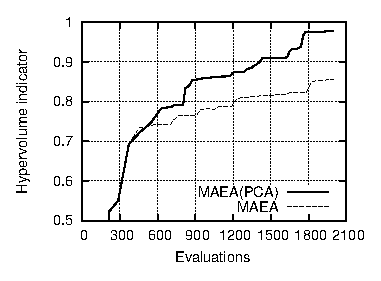
\includegraphics{nhyperv.eps}}
\end{minipage}
\begin{minipage}[b]{0.5\linewidth}
 \centering
 \resizebox*{7.0cm}{!}{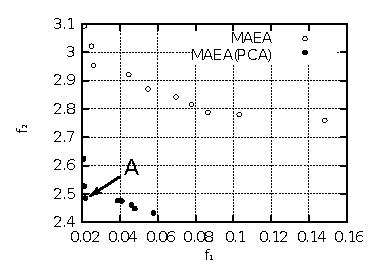
\includegraphics{fparetos.eps}}
\end{minipage}
\caption{Βελτιστοποίηση  υδροστροβίλου $Hydromatrix\circledR$: Σύγκριση της πορείας του δείκτη υπερόγκου για τους δικριτηριακούς ΜΑΕΑ και ΜΑΕΑ(\english{PCA}) (αριστερά). Μέτωπα μη-κυριαρχούμενων λύσεων για τις δύο μεθόδους που δοκιμάστηκαν επιβάλλοντας τερματισμό τους στις $2000$ αξιολογήσεις με το λογισμικό ΥΡΔ (δεξιά).}
\label{Matrix-Res}
\end{figure}

Το κέρδος από τη χρήση των προτεινόμενων τελεστών εξέλιξης υποβοηθούμενων από την ΑσΚΣ παρουσιάζεται στο σχήμα \ref{Matrix-Res}. Επίσης, παρουσιάζονται τα μέτωπα των μη-κυριαρχούμενων λύσεων που υπολογίστηκαν από τις δύο μεθόδους για το ίδιο υπολογιστικό κόστος ($2000$ αξιολογήσεις με το λογισμικό ΥΡΔ). Τέλος, από τα μέλη του μετώπου \english{Pareto} επιλέγεται ο σχεδιασμός Α και αναλύεται λεπτομερώς.  

Η ποιότητα του σχεδιασμού Α, όσον αφορά στην ποιότητα της φόρτισης και στη συνεργασιμότητα με τον αγωγό απαγωγής, παρουσιάζεται στο σχήμα \ref{Matrix-A} όπου απεικονίζονται τόσο οι κατανομές $C_p$ για τα τρία σημεία λειτουργίας που ενδιαφέρουν όσο και οι κατανομές των ταχυτήτων εξόδου $C_u$ και $C_m$. Στο ίδιο σχήμα εμπεριέχεται και πληροφορία για τη σπηλαίωση (λαμβάνεται από την ελάχιστη τιμή του $C_p$ για κάθε σημείο λειτουργίας) όπως, επίσης, και για την επιφάνεια άντλησης (διασταυρούμενες κατανομές $C_p$ στο σημείο ΜΦ).      

\begin{figure}[h!]
\begin{minipage}[b]{0.5\linewidth}
 \centering
 \resizebox*{6.5cm}{!}{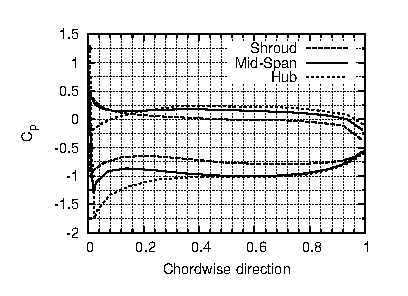
\includegraphics{LoadBE_M.eps}}
\end{minipage}
\begin{minipage}[b]{0.5\linewidth}
 \centering
 \resizebox*{6.5cm}{!}{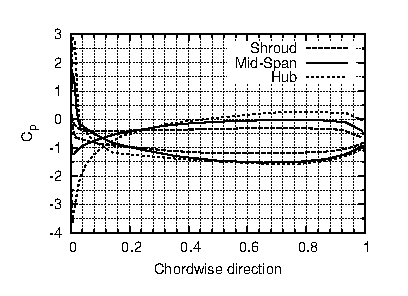
\includegraphics{LoadPL_M.eps}}
\end{minipage}
\begin{minipage}[b]{0.5\linewidth}
 \centering
 \resizebox*{6.5cm}{!}{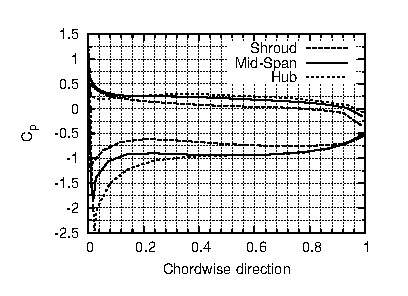
\includegraphics{LoadFL_M.eps}}
\end{minipage}
\begin{minipage}[b]{0.5\linewidth}
 \centering
 \resizebox*{6cm}{!}{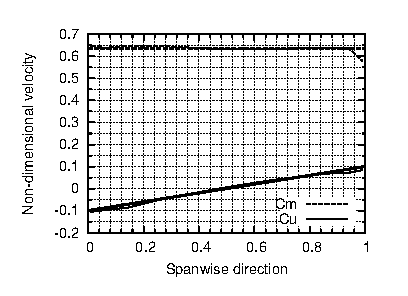
\includegraphics{OUTLETMATRIX.eps}}
\end{minipage}
\caption{Βελτιστοποίηση  υδροστροβίλου $Hydromatrix\circledR$: Κατανομές συντελεστή πίεσης ($C_p$) κατά μήκος της χορδής για το σχεδιασμό Α στα τρία σημεία λειτουργίας, ΜΑ (πάνω-αριστερά), ΜΦ (πάνω-δεξιά) και ΠΦ (κάτω-αριστερά). Κατανομές $C_u$ και $C_m$ για το σημείο ΜΑ, στην έξοδο του δρομέα, μαζί με τις χρησιμοποιηθείσες κατανομές-στόχους (κάτω-δεξιά).}
\label{Matrix-A}
\end{figure}

Η εμφάνιση επιφάνειας άντλησης γίνεται καλύτερα αντιληπτή στο σχήμα \ref{Matrix-A-2}. Οι γραμμές ροής κοντά στο κέλυφος στεφάνης (\english{shroud}) του δρομέα για το σημείο ΜΦ υποδηλώνουν ότι η ροή «συναντά» το πτερύγιο του δρομέα στην πλευρά υποπίεσης δημιουργώντας έτσι μία περιοχή υψηλότερων πιέσεων από τις αντίστοιχες στην πλευρά υπερπίεσης. Αυτή η ανεπιθύμητη συμπεριφορά δεν μπορεί να αποφευχθεί ε-ντελώς λόγω της φύσης του συγκεκριμένου τύπου υδροστρόβιλου αλλά η διαδικασία βελτιστοποίησης επιτυγχάνει τον περιορισμό της.       

\begin{figure}[h!]
\begin{minipage}[b]{0.5\linewidth}
 \centering
 \resizebox*{7cm}{!}{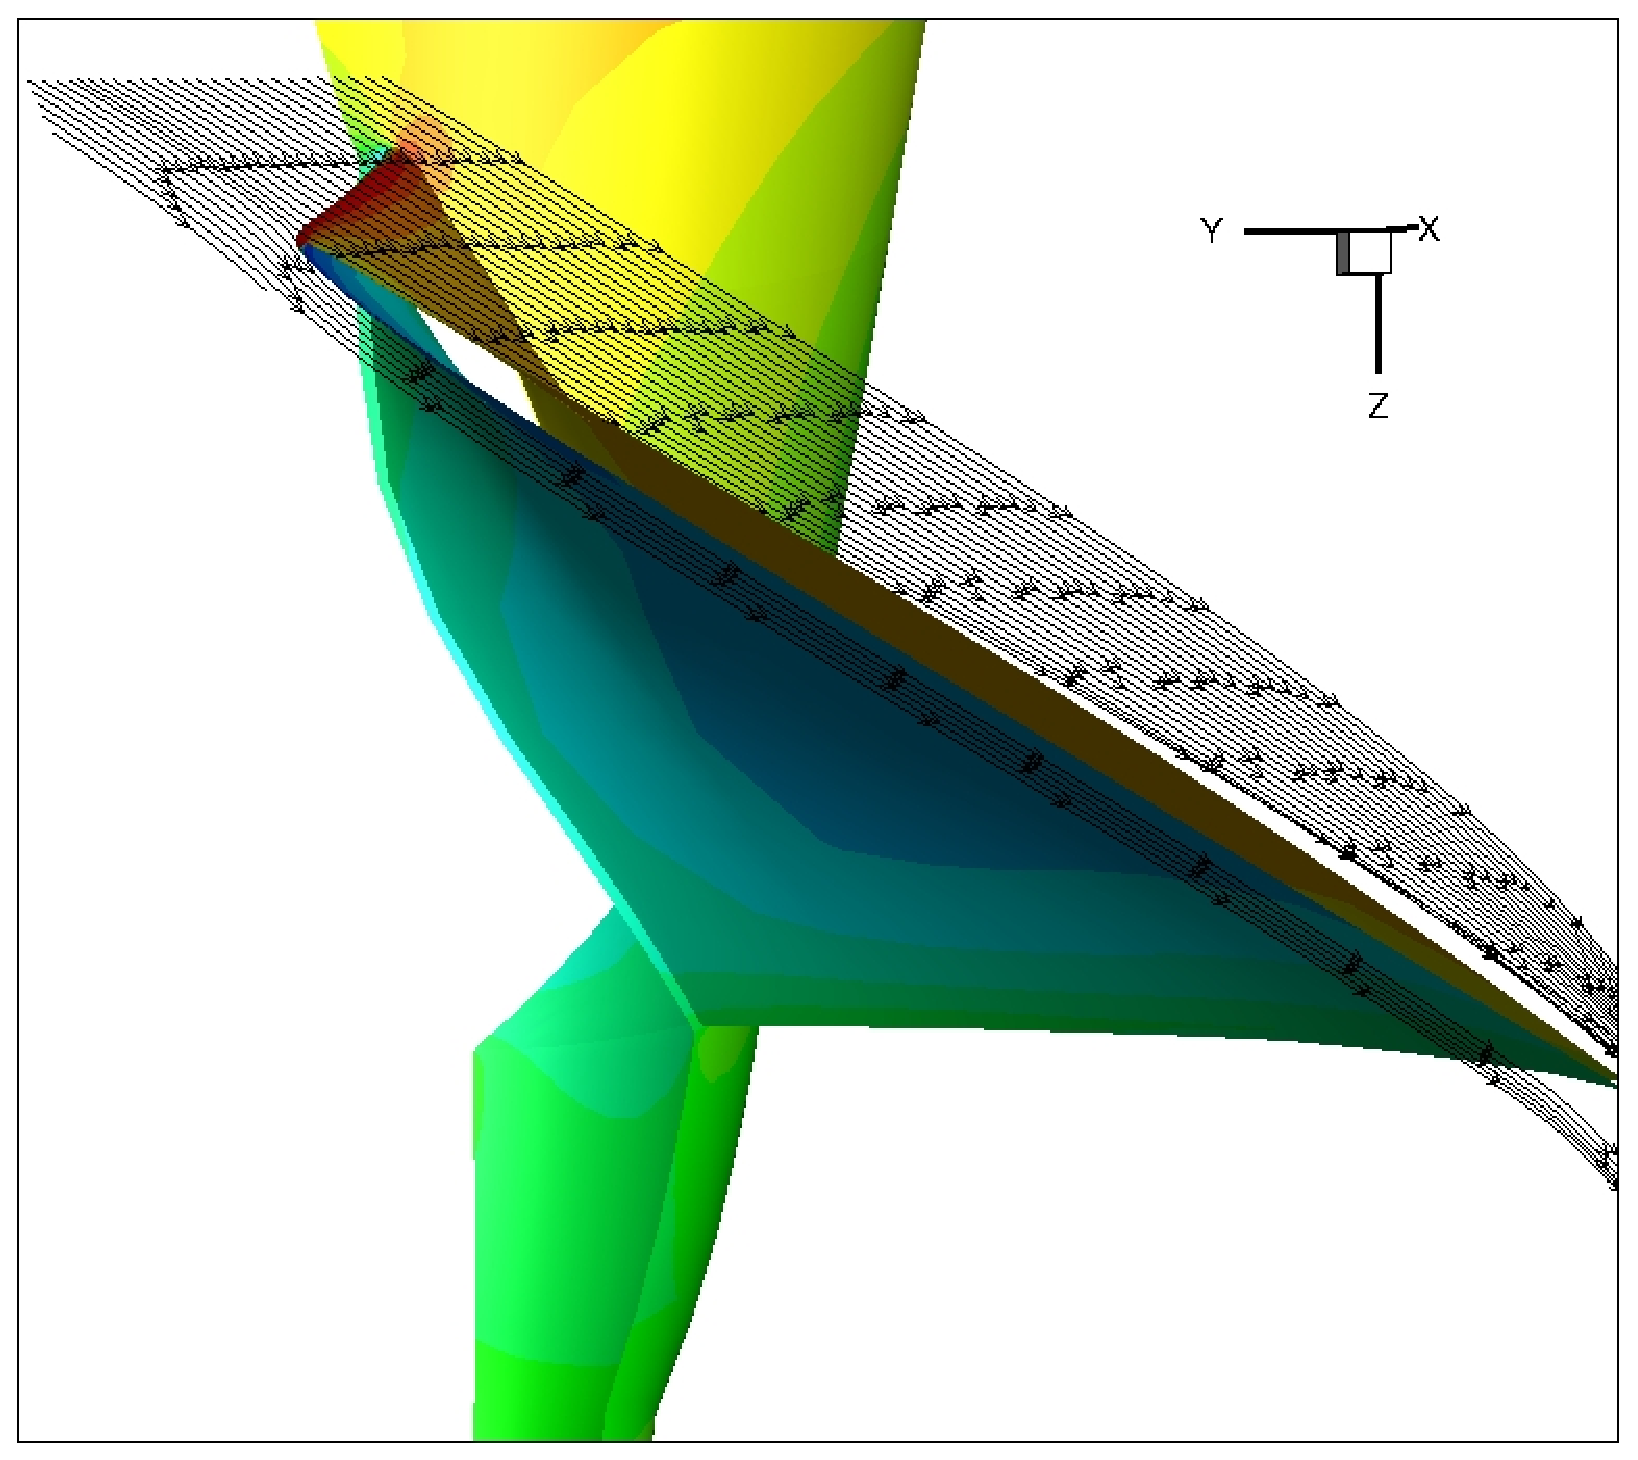
\includegraphics{BE.eps}}
\end{minipage}
\begin{minipage}[b]{0.5\linewidth}
 \centering
 \resizebox*{7cm}{!}{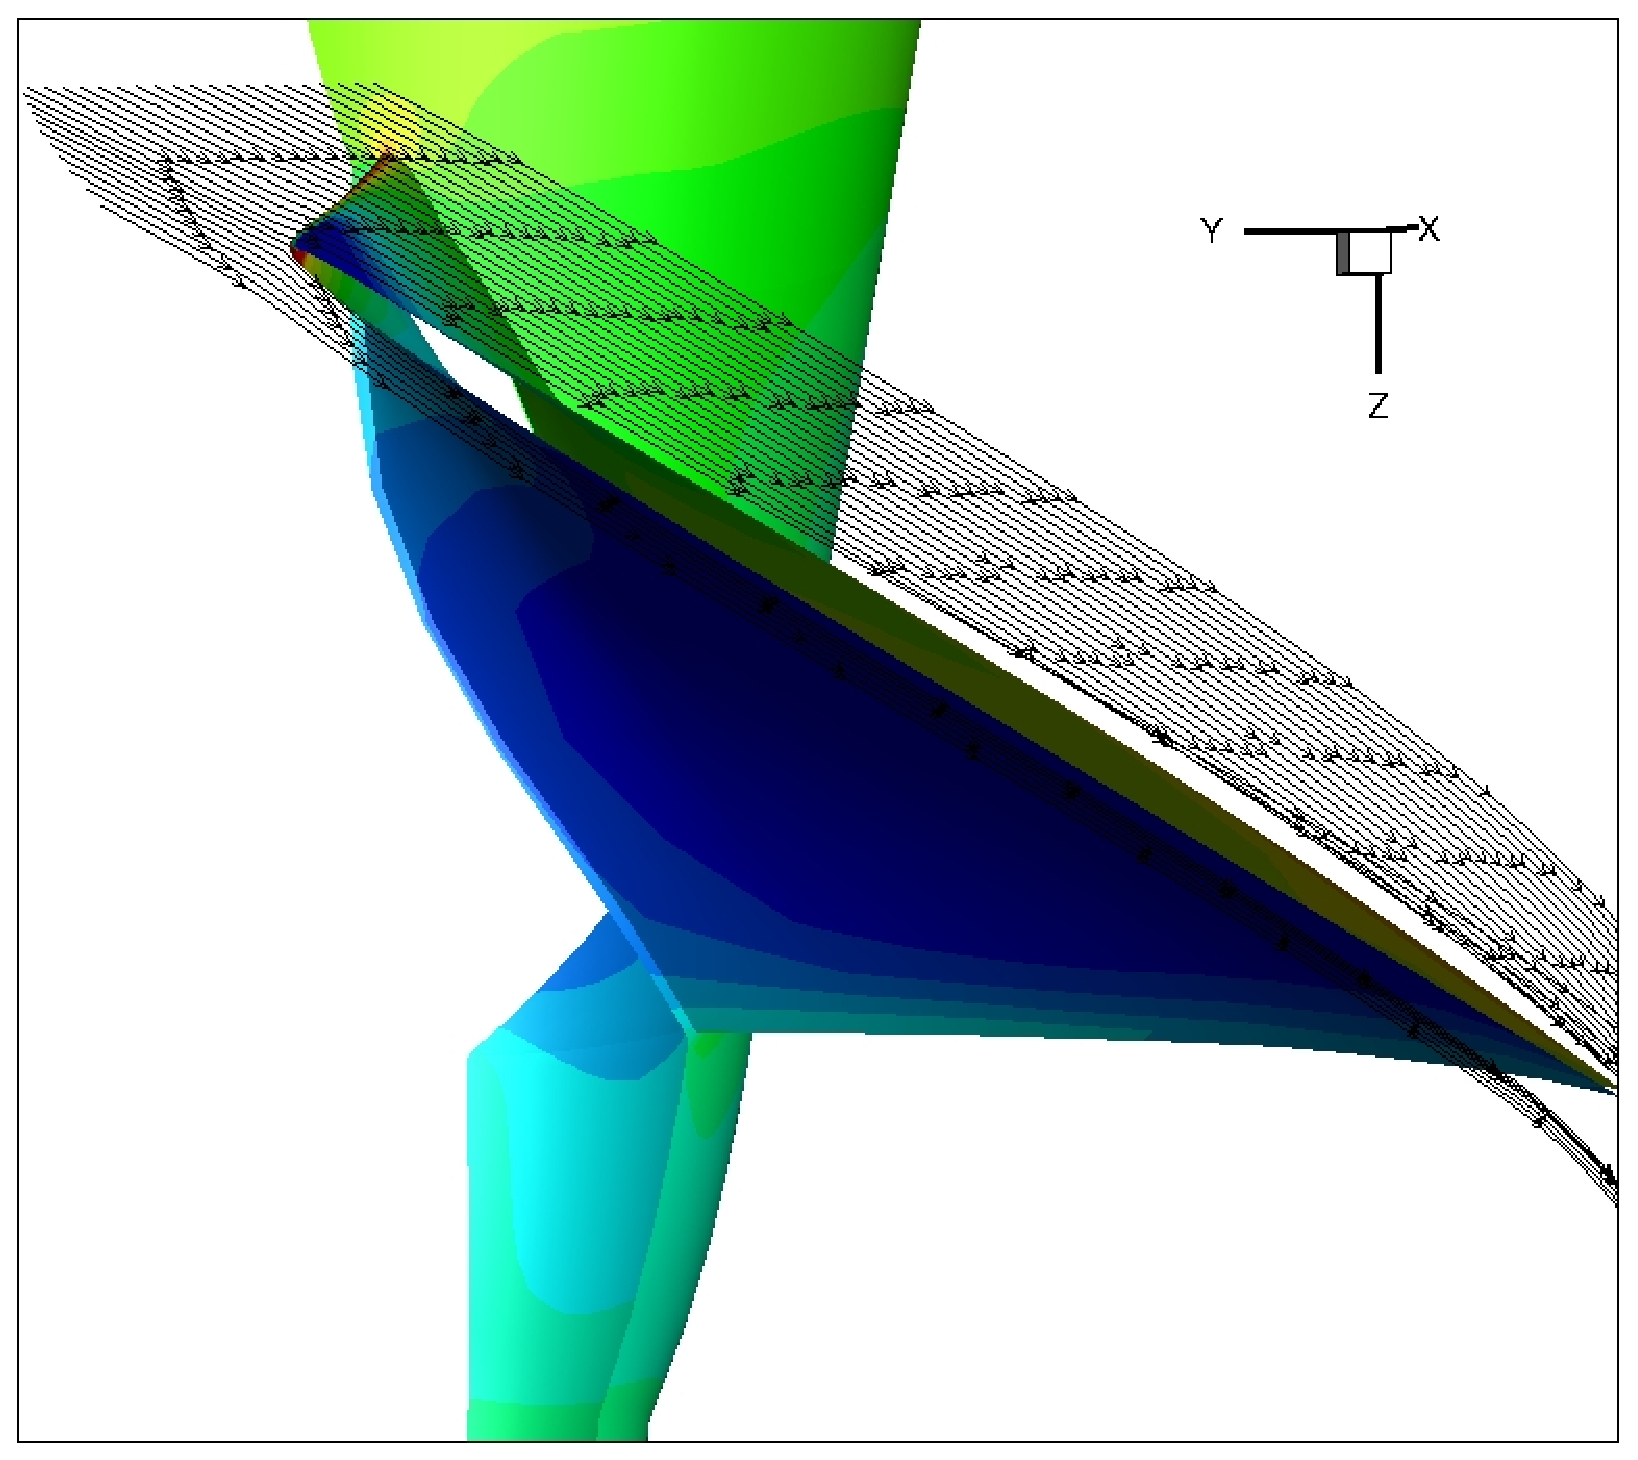
\includegraphics{PartLoad.eps}}
\end{minipage}
\begin{minipage}[b]{1\linewidth}
 \centering
 \resizebox*{7cm}{!}{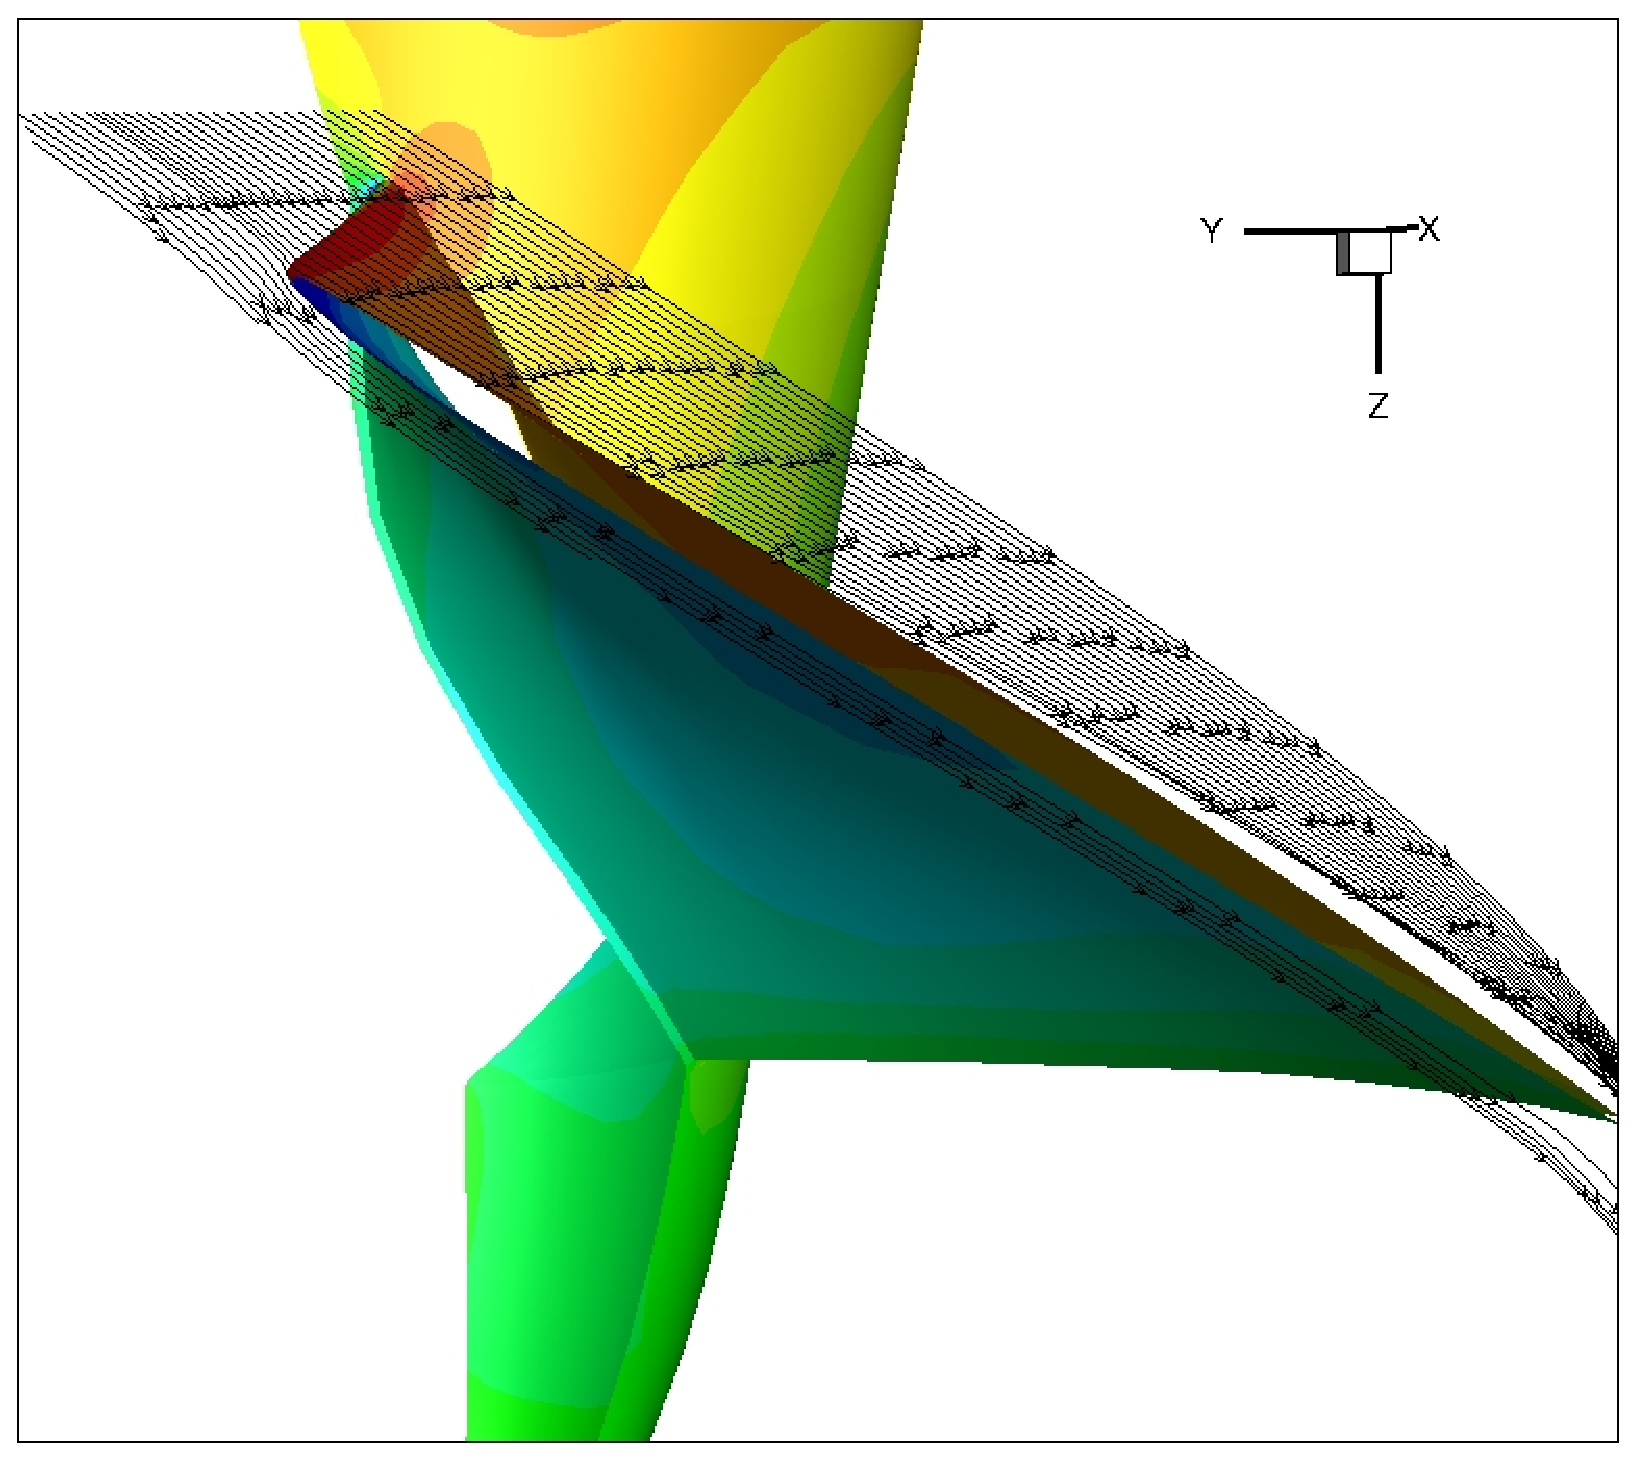
\includegraphics{FL.eps}}
\end{minipage}
\caption{Βελτιστοποίηση  υδροστροβίλου $Hydromatrix\circledR$: Ισοβαρείς επί της επιφάνειας του πτερυγίου και γραμμές ροής στην περιοχή του κελύφους στεφάνης (\english{shroud}) για το σχεδιασμό Α, μέλους του υπολογισθέντος μετώπου \english{Pareto}, στα τρία μελετούμενα σημεία λειτουργίας, ΜΑ (πάνω-αριστερά), ΜΦ (πάνω-δεξιά) και ΠΦ (κάτω).}
\label{Matrix-A-2}
\end{figure}


% ---------------------------------------------------------------------------
% ----------------------- end of thesis sub-document ------------------------
